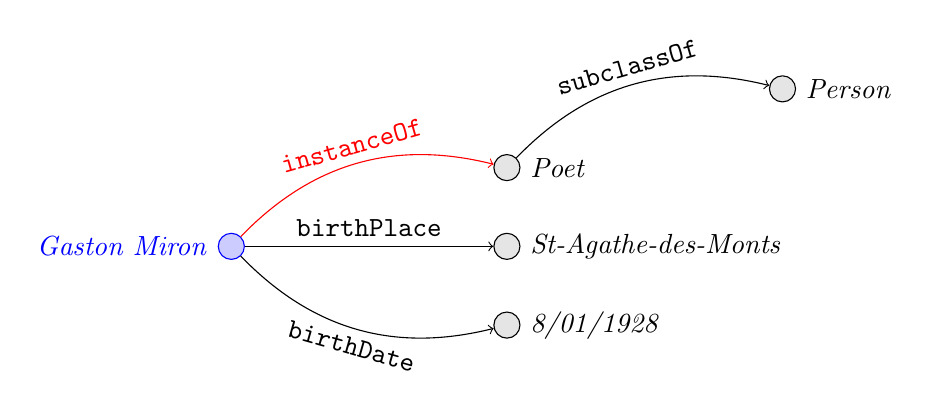
\begin{tikzpicture}
[   cnode/.style={draw=black,fill=#1,minimum width=3mm,circle},
    rnode/.style={draw=black,fill=#1,minimum width=6mm, minimum height=5mm, rectangle}
]
    

    \node[cnode=blue!20,draw=blue,label={[blue]180:\textit{Gaston Miron}}] (gm) at (0, 0) {};
    \node[cnode=gray!20, label=0:\textit{Poet}] (poet) at (3.5, 1) {};
    \node[cnode=gray!20, label=0:\textit{St-Agathe-des-Monts}] (sam) at (3.5, 0) {};
    \node[cnode=gray!20, label=0:\textit{8/01/1928}] (birth) at (3.5, -1) {};
    \node[cnode=gray!20, label=0:\textit{Person}] (sc) at (7, 2) {};
    
    \draw[->, red] (gm) to[bend left] node[midway, above, sloped]{\texttt{instanceOf}} (poet);
     \draw[->] (gm) -- node[midway, above]{\texttt{birthPlace}} (sam);
      \draw[->] (gm) to[bend right] node[midway, below, sloped]{\texttt{birthDate}} (birth);
       \draw[->] (poet) to[bend left] node[midway, above, sloped]{\texttt{subclassOf}} (sc);
    
\end{tikzpicture}